\section{Design}
\label{sec:design}
We describe the evolution of the design of \system{} starting with an initial strawman approach.  We then 
alter the design as we address each of the design goals discussed in the previous section, which brings us 
to a complete design.

\subsection{Strawman Approach: Hiding Information From CDN}
To prevent an inside attacker or government demanding data from learning information, the CDN 
must not have the knowledge of what content it is caching.  Therefore, the content {\it and} the 
associated URL must be obfuscated before it enters the CDN.  

{\bf Encrypt Content.}  The content can be obfuscated by encrypting it with a key that is not 
known to the CDN.  Because this must be done prior to any caching, the content publisher 
has to generate some key $k$ to encrypt the content with.  Then this encrypted (and subsequently 
obfuscated) content is then sent to the CDN, alternately pulled by the CDN, and stored in its caches.  
Additionally, if the domain supports HTTPS requests, then the content publisher must also encrypt the 
associated certificate with the same key $k$.  This content and certificate must be decrypted after 
it leaves the CDN; the client could decrypt the certificate and check its validity.  If valid, then 
the client uses $k$ to decrypt the content.  

{\bf Obfuscate URL.} Encrypting the content alone does not hide much from the CDN; the content 
identifier, or URL, must also be obfuscated, otherwise the CDN can still reveal information about 
which clients accessed which URLs (which is indicative of the content).  In order to obfuscate the 
URL, it too can be encrypted with key $k$ before it enters the CDN.  With encrypted content and 
URLs, the CDN does not know what content a given client is accessing.

{\bf Client Anonymization.}  The CDN may not know the content that a client is accessing, but it 
still knows information about the clients that are accessing any content at the CDN.  It knows 
where the clients are located and how many times they are accessing any content.  To address this, 
a client can simply use an anonymizing proxy or VPN when accessing content.  This hides a certain 
amount of information about the client, including the client's location and a direct link of 
client to content request.

This strawman approach obfuscates content from the viewpoint of the CDN, which also allows the CDN 
to claim plausible deniability when served with a subpoena.  Unfortunately, this approach has many 
limitations: are anonymizing proxies/VPNs trustworthy?, should clients be trusted to know $k$?, 
can any jurisdiction still subpoena the CDN for information (presumably the CDN has locations in many 
countries and clients in many countries)?, do malicious clients have more power as the CDN's attack 
detection and prevention capabilities are severely limited?

\subsection{Moving Jurisdictions}
As it is still unclear which jurisdiction is legally allowed to subpoena information from the CDN, this 
system should be a complement to the legal framework; it should make clear which jurisdictions are allowed 
which information, and also prevent an overreaching government from demanding data it should not have.  

{\bf Proxy in Client's Jurisdiction.}

{\bf Decouple Content Distribution from Decision of Trust.}

\subsection{Reducing Attack Surface}

{\bf Increasing the Number of Keys.}

{\bf Introducing Randomness to URL Obfuscation.}

\begin{figure}[h]
\centering
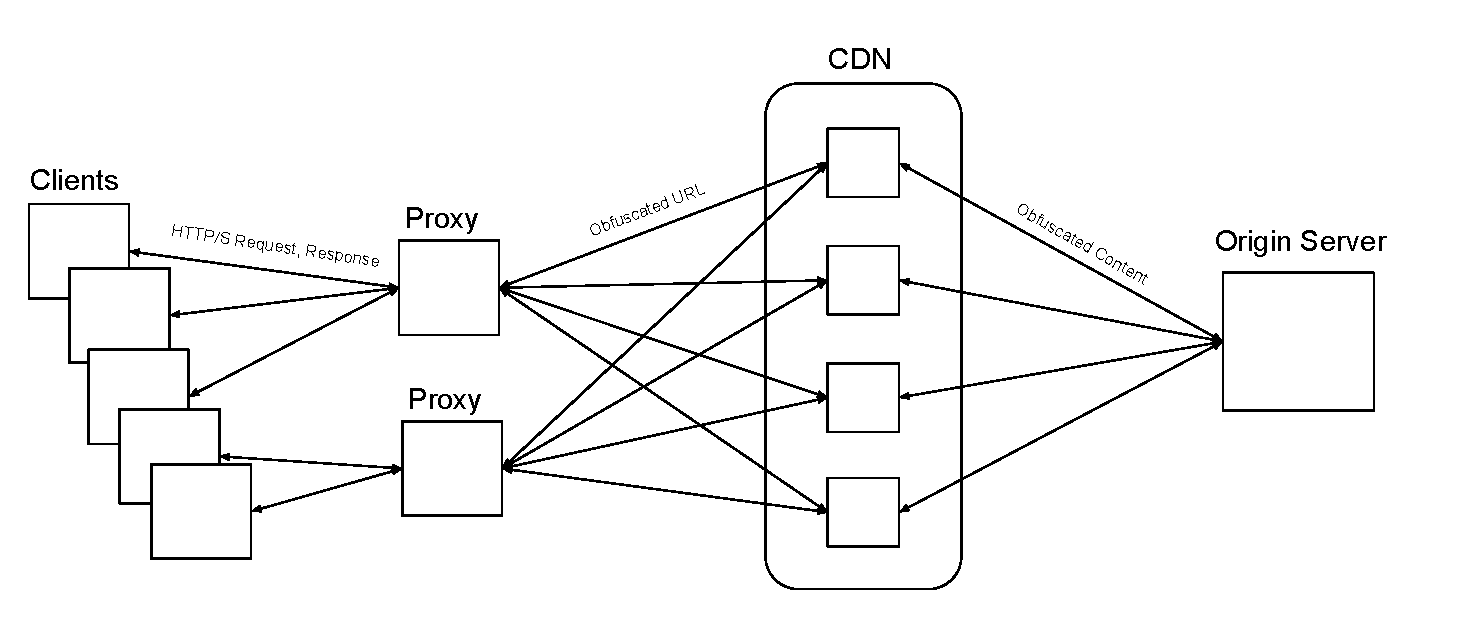
\includegraphics[width=.5\textwidth]{full_ocd_system}
\caption{The relationships between clients, the CDN, proxies, and content publishers in 
\system{}.}
\label{fig:ocd_overview}
\end{figure}
